\documentclass[xcolor=dvipsnames,aspectratio=169,t]{beamer}
  % t means frames are vertically centered to the top
\usepackage{slides-header}
\title{The Matrix of a Linear Transformation}

\begin{document}
\maketitle

\begin{frame}{The Matrix of a Linear Transformation}

  Let $T: \mathbb{R}^3 \to \mathbb{R}^4$ denote a linear transformation with
  \[ \colorg{T \left( \begin{bmatrix} 1\\0\\0 \end{bmatrix} \right) = T(\mathbf{e}_1) = \begin{bmatrix} 3\\-1\\1\\0\end{bmatrix}}  \ , \ \ \colorr{T \left( \begin{bmatrix} 0\\1\\0 \end{bmatrix} \right) = T( \mathbf{e}_2) = \begin{bmatrix} 0\\2\\1\\3\end{bmatrix}} \ , \ \ \colorb{T \left( \begin{bmatrix} 0\\0\\1 \end{bmatrix} \right) = T(\mathbf{e}_3) = \begin{bmatrix} 1\\0\\1\\-1\end{bmatrix}} .\]\

  Find the image of an \alert{arbitrary vector $\mathbf{x}$} in  $\mathbb{R}^3$.

  \pause
  \begin{align*}
  T(\mathbf{x}) &= T\left( x_1 \mathbf{e}_1 + x_2 \mathbf{e}_2 + x_3 \mathbf{e}_3 \right) = x_1 \colorg{T(\mathbf{e}_1)} + x_2 \colorr{T(\mathbf{e}_2)}  + x_3 T(\colorb{\mathbf{e}_3})  \\
  &= x_1 \colorg{\begin{bmatrix} 3\\-1\\1\\0\end{bmatrix}} + x_2  \colorr{\begin{bmatrix} 0\\2\\1\\3\end{bmatrix}}  + x_3  \colorb{\begin{bmatrix} 1\\0\\1\\-1\end{bmatrix} } 
  = \begin{bmatrix} \colorg{3} & \colorr{0} & \colorb{1} \\ \colorg{-1} & \colorr{2} & \colorb{0} \\ \colorg{1} & \colorr{1} & \colorb{1} \\ \colorg{0} & \colorr{3} & \colorb{-1} \end{bmatrix} \begin{bmatrix}x_1\\x_2\\x_3 \end{bmatrix} 
  = A \x.
  %= \begin{bmatrix} 3x_1+x_3\\ -x_1+2x_2 \\ x_1+x_2+x_3\\ 3x_2-x_3 \end{bmatrix}
  \end{align*}

\end{frame}


\begin{frame}{Every Linear Transformation is a Matrix Transformation}

\begin{theorem}
For any linear transformation $T\colon\R^n \to \R^m$, there is a unique matrix $A$ (called the \alert{associated matrix for the linear transformation}) such that $T(\mathbf{x}) = A \mathbf{x}$ for all $\mathbf{x}$ in $\mathbb{R}^n$.  The matrix $A$ can be found by
\[ A = \begin{bmatrix} T\left(\mathbf{e}_1 \right) & T\left(\mathbf{e}_2 \right) & \ldots & T\left(\mathbf{e}_n \right) \end{bmatrix}.\]

\end{theorem}

  \pause
  \begin{proof}
  \begin{align*}
  T(\mathbf{x}) &= T \left( x_1 \mathbf{e}_1 + x_2 \mathbf{e}_2 + \ldots + x_n \mathbf{e}_n \right) 
  = x_1 T \left( \mathbf{e}_1 \right) + x_2 T \left( \mathbf{e}_2 \right) + \ldots + x_n T \left( \mathbf{e}_n \right) \\
  &= \begin{bmatrix}  T \left( \mathbf{e}_1 \right)  & T \left( \mathbf{e}_2 \right) & \ldots & T \left( \mathbf{e}_n \right) \end{bmatrix} \begin{bmatrix} x_1 \\  \vdots \\ x_n \end{bmatrix} 
  = A \mathbf{x}.
  \end{align*}
  \end{proof}
\end{frame}

\begin{frame}{Geometric Interpretation in $\mathbb{R}^2$}

Consider the linear transformation given by $T: \mathbb{R}^2 \to \mathbb{R}^2: \mathbf{x} \mapsto 0.5 \mathbf{x}$. Find the associated matrix $A$ for this linear transformation. \bs

We have  $\dsty \alert{T(\mathbf{e}_1) = \begin{bmatrix} 0.5 \\ 0 \end{bmatrix}}$ and $\dsty \colorb{T(\mathbf{e}_2) = \begin{bmatrix} 0 \\ 0.5 \end{bmatrix}}$ giving the matrix $\dsty A = \begin{bmatrix} \alert{0.5} & \colorb{0} \\ \alert{0} & \colorb{0.5} \end{bmatrix}$.

\begin{columns}

\column{0.33\tw}

\begin{center}
\includegraphics[width=0.8\tw]{images/fig-ele-pic.JPG}
\end{center}

\column{0.33\tw}

\begin{center}
\includegraphics[width=0.8\tw]{images/fig-elephant.png}
\end{center}

\column{0.33\tw}

\begin{center}
\includegraphics[width=0.8\tw]{images/fig-ele-dilate.png}
\end{center}

\end{columns}

\end{frame}

\begin{frame}{Geometric Interpretation in $\mathbb{R}^2$}

Consider the linear transformation given by $\dsty T(\mathbf{x}) = A \mathbf{x} = \begin{bmatrix} -1 & 0 \\ 0 & 1 \end{bmatrix}\x$. 

We have  $\dsty \alert{T(\mathbf{e}_1) = \begin{bmatrix} -1 \\ 0 \end{bmatrix}}$ and $\dsty \colorb{T(\mathbf{e}_2) = \begin{bmatrix} 0 \\ 1 \end{bmatrix}}$ giving the geometric interpretation seen below.

\begin{columns}

\column{0.5\tw}

\begin{center}
\includegraphics[width=0.6\tw]{images/fig-elephant.png}
\end{center}

\column{0.5\tw}

\begin{center}
\includegraphics[width=0.6\tw]{images/fig-ele-reflect.png}
\end{center}

\end{columns}

\end{frame}

\begin{frame}{Contractions and Expansions}

Consider the linear transformation given by $\dsty T(\mathbf{x}) = A \mathbf{x} = \begin{bmatrix} 1 & 0 \\ 0 & 2 \end{bmatrix}\x$. 

We have  $\dsty \alert{T(\mathbf{e}_1) = \begin{bmatrix} 1 \\ 0 \end{bmatrix}}$ and $\dsty \colorb{T(\mathbf{e}_2) = \begin{bmatrix} 0 \\ 2 \end{bmatrix}}$ giving the geometric interpretation seen below.

\begin{columns}

\column{0.5\tw}

\begin{center}
\includegraphics[width=0.6\tw]{images/fig-elephant2.png}
\end{center}

\column{0.5\tw}

\begin{center}
\includegraphics[width=0.6\tw]{images/fig-ele-expand.png}
\end{center}

\end{columns}

\end{frame}

\begin{frame}{Shear Transformations}

Consider the linear transformation given by $\dsty T(\mathbf{x}) = A \mathbf{x} = \begin{bmatrix} 1 & 0.75 \\ 0 & 1 \end{bmatrix}\x$. 


\begin{columns}

\column{0.5\tw}

\begin{center}
\includegraphics[width=0.6\tw]{images/fig-elephant.png}
\end{center}

\column{0.5\tw}

\begin{center}
\includegraphics[width=0.6\tw]{images/fig-ele-shear.png}
\end{center}

\end{columns}

\end{frame}

\begin{frame}{Projections}

Consider the linear transformation given by $\dsty T(\mathbf{x}) = A \mathbf{x} = \begin{bmatrix} 1 & 0 \\ 0 & 0 \end{bmatrix}\x$. 


\begin{columns}

\column{0.5\tw}

\begin{center}
\includegraphics[width=0.6\tw]{images/fig-elephant.png}
\end{center}

\column{0.5\tw}

\begin{center}
\includegraphics[width=0.6\tw]{images/fig-ele-project.png}
\end{center}

\end{columns}
\end{frame}

\begin{frame}{Rotations}
\medskip

  Consider the linear transformation $T$ of $\mathbb{R}^2$ that rotates by the angle $\theta$.
  What is the associated matrix of $T$?
  
  \pause
  \begin{columns}
  \column{0.65\tw}
    \begin{center}
    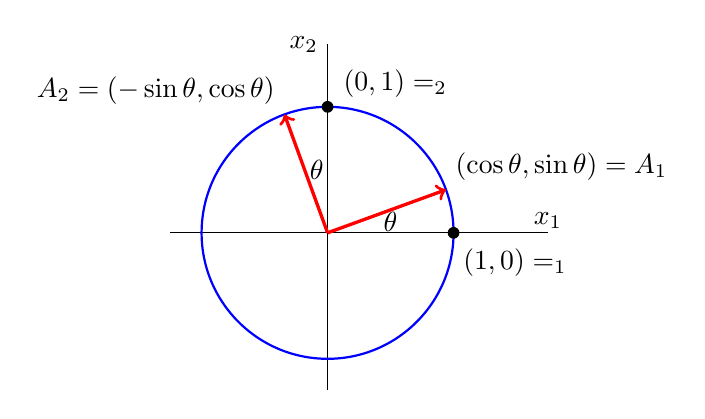
\begin{tikzpicture}[scale=1.6]
      \draw (-1.25,0)--(1.75,0);
      \draw (0,-1.25,0)--(0,1.5);
      \draw[blue,thick] (0,0) circle (1);
      % theta is 20 degrees
      \draw[red,very thick,->] (0,0)--(0.9396926207859084,0.3420201433256687);
      \node[anchor=south west] at (0.9396926207859084,0.3420201433256687) {$(\cos \theta,\sin \theta)=A\e_1$};
      \node at (.5,.085) {$\theta$};
      \node at (1.75,.1) {$x_1$};
      \node[anchor=north west] at (1,-.05) {$(1,0)=\e_1$};
      \node at (1,0)[circle,fill,inner sep=1.5pt]{};
      
      \onslide<3->{
      \draw[red,very thick,->] (0,0)--(-0.3420201433256687,0.9396926207859084);
      \node[anchor=south east] at (-0.3420201433256687,0.9396926207859084) {$A\e_2=(-\sin \theta,\cos \theta)$};
      \node at (-.085,.5) {$\theta$};
      \node[anchor=south east] at (0,1.35) {$x_2$};
      \node[anchor=south west] at (.05,1) {$(0,1)=\e_2$};
      \node at (0,1)[circle,fill,inner sep=1.5pt]{};
      }
    \end{tikzpicture}
    \end{center}

  \column{0.35\tw}
    \vspace*{3em}
    
    $T(\mathbf{x})= A\mathbf{x}= 
    \begin{bmatrix} \cos \theta & \onslide<3->{ -\sin \theta } \\ 
                    \sin\theta & \onslide<3->{\cos\theta} \end{bmatrix}\mathbf{x}$
  \end{columns}
\end{frame}


\begin{frame}{Properties of Linear Transformations}

\bbox
Let $T: \mathbb{R}^n \to \mathbb{R}^m$ be a linear transformation. The mapping $T$ is said to be:

\bi
\ii  \alert{One-to-one} if each $\mathbf{b}$ in $\mathbb{R}^m$ has \textbf{at most one} $\mathbf{x}$ in $\mathbb{R}^n$ such that $T( \mathbf{x}) = \mathbf{b}$.
\ii \alert{Onto} if each $\mathbf{b}$ in $\mathbb{R}^m$ is the image of \textbf{at least one} $\mathbf{x}$ in $\mathbb{R}^n$ such that $T( \mathbf{x}) = \mathbf{b}$.
\ei

\ebox

  \pause
  \begin{example}
  \bi 
  \ii The dilation transformation $\dsty T(\mathbf{x}) =  \begin{bmatrix}  0.5 & 0 \\ 0 & 0.5 \end{bmatrix} \begin{bmatrix} x_1 \\ x_2 \end{bmatrix}$ is both one-to-one and onto.
  \medskip
  \ii The projection transformation $\dsty T(\mathbf{x}) =  \begin{bmatrix}  1 & 0 \\ 0 & 0 \end{bmatrix} \begin{bmatrix} x_1 \\ x_2 \end{bmatrix}$ is neither one-to-one nor onto.
  \ei
  \end{example}

\end{frame}

\begin{frame}{Examples}

Determine whether each of the transformations is one-to-one and/or onto. 

\begin{columns}[T]

\column{0.33\tw}

$\dsty T: \mathbb{R}^3 \to \mathbb{R}^2: \begin{bmatrix} x_1\\x_2\\x_3 \end{bmatrix} \mapsto \begin{bmatrix} x_1 \\ x_2 \end{bmatrix}$

\column{0.34\tw}

$\dsty R: \mathbb{R}^3 \to \mathbb{R}^3: \begin{bmatrix} x_1\\x_2\\x_3 \end{bmatrix} \mapsto \begin{bmatrix} -x_2 \\ -x_3 \\ -x_1 \end{bmatrix}$

\column{0.33\tw}

$\dsty S: \mathbb{R}^2 \to \mathbb{R}^3: \begin{bmatrix} x_1\\x_2 \end{bmatrix} \mapsto \begin{bmatrix} x_2 \\ 0 \\ x_1 \end{bmatrix}$

\end{columns}

\vspace{3in}

\end{frame}

\begin{frame}

{\small
\begin{theorem}
A linear transformation $T: \mathbb{R}^n \to \mathbb{R}^m$ is \colorr{one-to-one} if and only if $T(\mathbf{x}) = \mathbf{0}$ has only the \colorb{trivial solution}.
\end{theorem}

\smallskip

\begin{proof}
  \pause
  The forward direction we prove using proof by contradiction. Let's assume that $T$ is a one-to-one mapping, and that $T(\mathbf{x})=\mathbf{0}$ has a non-trivial solution $\mathbf{v}$ in $\mathbb{R}^n$.
  Then $T$ is not one-to-one since $T(\mathbf{0}) = T(\mathbf{v}) = \mathbf{0}$.
  Thus we have a contradiction.
  \medskip

  \pause
  The reverse direction we prove using proof by contradiction as well. Suppose $T(\mathbf{x}) = \mathbf{0}$ has only the trivial solution, and $T$ is not one-to-one. This means there exist $\mathbf{u} \ne \mathbf{v}$ both in $\mathbb{R}^n$ with $T(\mathbf{u})=T(\mathbf{v}) = \mathbf{b}$ in $\mathbb{R}^m$. 
  \pause
  Therefore, we have
  \[  T(\mathbf{u} -\mathbf{v}) = T(\mathbf{u}) - T(\mathbf{v}) = \mathbf{b} - \mathbf{b} = \mathbf{0}.\]
  Since $\mathbf{u} \ne \mathbf{v}$, we have found a non-trivial solution such that $T(\mathbf{u} -   \mathbf{v}) = \mathbf{0}$.
  Thus we have a contradiction.
\end{proof}
}

\end{frame}

\begin{frame}{Summary}

\bbox
A linear transformation $T: \mathbb{R}^n \to \mathbb{R}^m$ with associated matrix $A$ is \alert{one-to-one} if and only if 

\bi
\ii $T(\mathbf{x}) = \mathbf{0}$ has only the trivial solution.
\ii The solution set to $A \mathbf{x} = \mathbf{0}$ has no free variables.
\ii The matrix $A$ has a pivot in every column.
%\ii \alert{The columns of $A$ are linearly independent.}
\ei
\ebox

\bbox
A linear transformation $T: \mathbb{R}^n \to \mathbb{R}^m$ with associated matrix $A$ is \colorb{onto} if and only if 

\bi
\ii For any $\mathbf{b}$ in $\mathbb{R}^m$ there exists at least one $\mathbf{x}$ in $\mathbb{R}^n$ with $A \mathbf{x} = \mathbf{b}$.
\ii All vectors $\mbf{b}$ in $\mathbb{R}^m$ can be written as a linear combination of the columns of $A$.
\ii The matrix $A$ has a pivot in every row.
\ii \colorb{The columns of $A$ span all of $\mathbb{R}^m$.}
\ei
\ebox

\end{frame}

\end{document}
